\label{sec:patterns}

\subsection{Defining pattern reproduction}

After making the observations in the previous section the next question that naturally occurs is if given a certain pattern, is there an associated graph topology (or associated matrix $A$) that is capable of reproducing it? In other words given a pattern, can we ``train'' a topology to create it?

In order to answer this question we first need to define ``pattern'' properly. We consider a pattern as the set of phase shifts between the different Kuramoto oscilators. In order to be able to observe a pattern it is neccessary for the oscilators to either have the same intrinsic frequencies $\omega_i$ or lock into the same frequency. In our case we just consider the first case. 

The reader should furthermore note that since we only consider phase shifts, the order of oscilators themselves is not relevant and all observation should be invariantmodulo $2\pi$. 

\subsection{Simple patterns}

We shall first consider the simple case of reproducing a simple pattern between 2 oscilators. If we take into account what we learned in the previous section, it is easily possible to re-create phase-shifts of $\frac{2\pi}{p}$ when $p$ is prime. 

If we set up $p$ oscilators on a cylic graph, we can get different phase shifts between neighbouring oscilators. For each divisor $d \neq 1$ of $p$ we can achieve phase shifts of $\frac{2\pi}{d}$ between neighbouring nodes. However since $p$ is prime, there is only a single such divisor, namely $p$ itself, and we will always achieve a phase shifts of $\frac{2\pi}{p}$. 

There is a caveat to this situation: We now have $p$ different oscilators in our topology instead of just two. This is not a big problem however, we can just pick two oscilators at random and ignore the others. 

\subsection{Creating More Complex Patterns}

We now have the ability to create simple patterns by setting up oscilators in a cirle topology. Using the same topology we can also create offsets of the shape $\frac{a {\cdot} 2 \pi}{p}$ where $p$ prime and $a \in \mathbb{N}$. Instead of taking two neighbouring nodes, we can just take two nodes of distance $A$ on the same topology. 

This introduces yet another caveat to the situation: We know the phase shift difference between two values but we can not predict which one is of higher value and which one is of lower value. Since we are working modulo $2 \pi$ this is not even well defined. 

But how can we expand this behaviour to reproduce any phase shifts $\frac{p {\cdot} 2 \pi}{q}$ with $p, q \in \mathbb{N}, q \neq 0$? Turns out it is possible to ``add'' phase shifts by joining two cicular toplogies. Both circles will behave as they would individually and additionally the node at which they are joined will always have the same value. 

If we wanted to for example reproduce the phase $\frac{8 {\cdot} 2 \pi}{15}$ we can use one circle of size $3$ and one circle of size $5$. Their phase shifts of $\frac{2\pi}{5}$ and $\frac{2\pi}{5}$ add up to $\frac{8 {\cdot} 2 \pi}{15}$, exactly what we want. The topology can bee seen in Figure~\ref{fig:pattern_joined}. 

\begin{figure}[h]
  \centering
  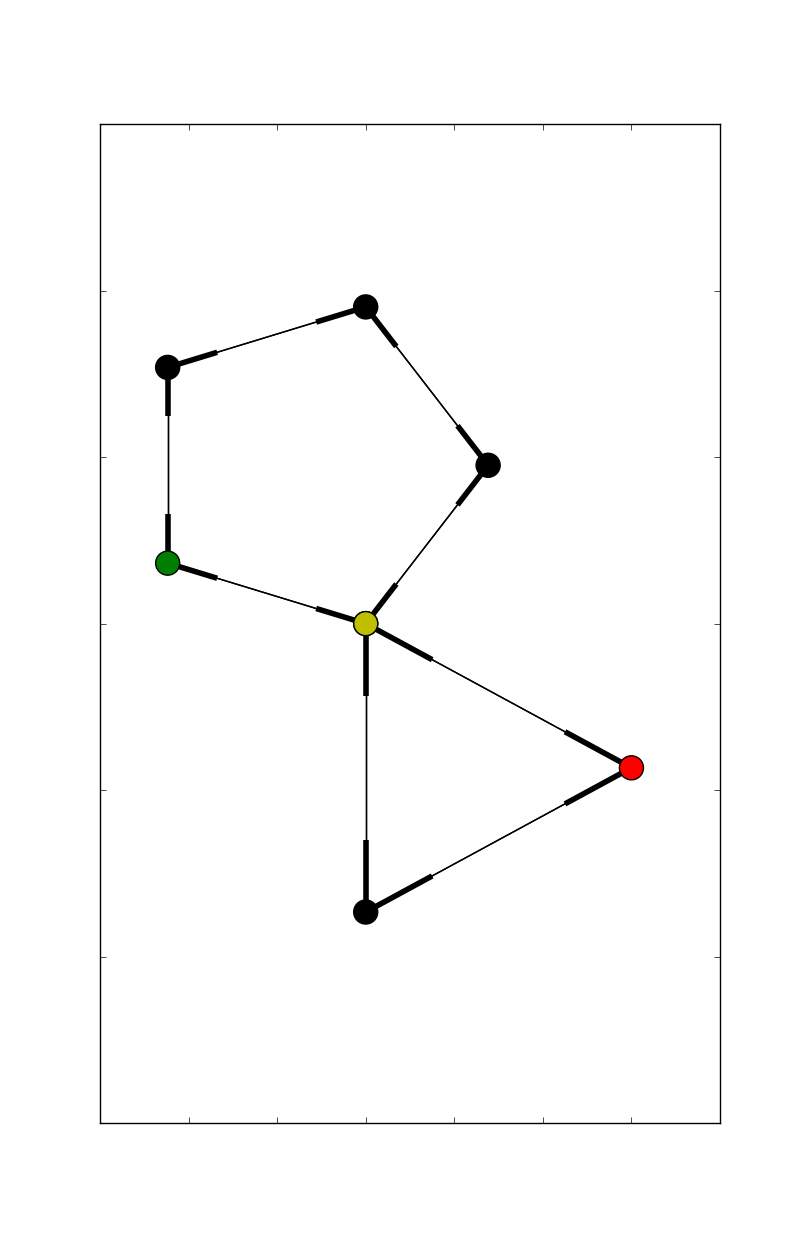
\includegraphics[height=0.5\textheight]{imgs/pattern_joined}
  \caption{Graph topology used to reproduce a more complex pattern: Two cicular topologies joined at the yellow node. The green and yellow nodes will have a phase shift of $\frac{2\pi}{5}$, the yellow and red nodes will have a phase shift of $\frac{2\pi}{3}$. This gives a total phase shift of $\frac{2\pi}{5} + \frac{2\pi}{5} = \frac{8 {\cdot} 2 \pi}{15}$. }
  \label{fig:pattern_joined}
\end{figure}

There is however a slight problem still: We have no guarantee that the total phase shift is indeed the sum of phase shifts in the individual circles. Since the phase shifts could propagnate in different directions the total phase shift could actually be the difference. We can work around this however by choosing the correct initial values for the oscilators -- both states are equally stable. 

Finally we can note that it is possible to further expand these patterns. Instead of just two circles, we can take more circles to produce offsets of the form

\[
  \sum_{i}{\frac{q_i {\cdot} 2 \pi}{p_i}}
\]

with $p_i$ prime and $q_i \in \mathbb{N}$. In fact if we take into account that we are operating modulo $2 \Pi$ we can even take $q_i \in \mathbb{Z}$. 
Now given any phase shift $\frac{p {\cdot} 2 \pi}{q}$ we can obviously use the prime factors as denominators $p_i$ and write it in this form. We can then use the procedure described above to create a topology that can produce the given phase shift. 

If we have more than two oscilators in a pattern that we want to construct, we can also continue this procedure. We can just join more circles to the node we want to define a phase shift relative to. 